\documentclass[conference]{IEEEtran}
% Packages
%\pdfobjcompresslevel=0
\usepackage{titlesec}
\usepackage{graphicx}
\usepackage{lipsum} % For dummy text, you can remove this
\usepackage[style=numeric, backend=biber]{biblatex} % Import the package for reading .bib files
\addbibresource{Communication.bib} % Add the .bib file
\usepackage{algorithm}
\usepackage{algpseudocode}
\usepackage{booktabs}
\usepackage{float}
\usepackage{multirow}

% Title page
\title{Dissertation Title}
\author{Luis Yallico Ylquimiche}
\date{\today}

\begin{document}

% Title page
\maketitle

% Abstract
\begin{abstract}
LOREM IPSUM
\end{abstract}


\section{Introduction}

Swarm engineers draw inspiration from social biological systems such as ants or bees to build decentralised robot collectives that are inherently robust to failure, flexible across tasks and scalable in number \cite{dias_swarm_2021}. In swarm systems, collective intelligence emerges when individual robots trade packets of information among neighbouring robots. Classic ant-colony-optimisation (ACO) work in the early 2000s has already proven that an indirect information exchange "virtual-pheromones" can lead to agents collectively discovering optimal routing behaviours \cite{dorigo_ant_2000}. Highlighting the importance of communication design in swarms and the effect it can have over their behaviour.\\

While coordination and task allocation have been widely studied, recent surveys highlight bandwidth, latency and energy usage as key limitations to real-world swarm deployments \cite{an_multi-robot_2023}\cite{ding_advancements_2023}. These issues become more pronounced as swarm sizes scale, resulting in an increase in data volume being transmitted among swarm peers, often overwhelming individual agents' hardware capabilities.\\

Beyond the swarm's exchange capacity, the architecture of the communication also matters. In many direct communication schemes, broadcasting is a common mode of data transmission across various swarm deployments \cite{an_multi-robot_2023}. For example,\cite{perrin_decentralised_2012} demonstrated that peer-to-peer broadcasts allowed swarms to map unknown environments in disaster zones. However, this type of data flooding is known to scale poorly \cite{an_multi-robot_2023}, this due to increasing Wi-Fi collision rates once swarms grow past a few dozen peers.\\ 

Furthermore, embodied evolution of swarm controllers heavily relies on communication to tune the controller. Some recent studies explain that less communication can sometimes enhance swarm performance, as trimming neighbourhood size helps populations forget outdated beliefs and re-adapt faster \cite{hiraga_when_2023}\cite{ding_advancements_2023}. Most of these studies were performed in simulation, hence the need for empirical data on how swarm density, rate of data transfer and packet content affects evolution performance. With this in mind, it is possible to think of communication as a dynamic resource that can be manipulated by the swarm to achieve its goals. The ways in which this resource is allocated can have a significant impact on the behaviour of the swarm.\\

This study profiles swarm communication on ESP32 hardware, evaluating performance under varied conditions such as agent density, locomotion, topology inference, imposed message budgets and stochastic transmission. With a focus on direct peer-to-peer communication  we aim to (i) provide empirical data to validate the challenges flagged by literature, and (ii) inform tangible communication design rules for future swarm systems.

\section{Related Work}

%add This is based on the Island model [ref], where different subpopulations (islands) evolve in parallel and occasionally exchange individuals (migration) with other islands, thus enabling the swarm to converge to a solution. 

%We utilized the built-in WiFi capabilities of the ESP32 with the ESPNOW communication protocol, which supports multiple unicast connections. While ESPNOW can theoretically handle around 20 devices simultaneously, practical limits are dictated by environmental factors. Additionally, ESPNOW enables multicast data transmission to multiple devices on the same channel, which can be used to pair devices or send messages to multiple swarm members. The protocol operates at a default bitrate of approximately 1 Mbps, although a portion of this bandwidth is consumed by necessary overhead, such as the MAC header. 

%For expanding a swarm dynamically, cryptographic keys might be needed to securely onboard new members, this however is out of scope of the current study.

%one way communication

\section{Experimental Setting}

In this study, a global optimisation problem known as the Rastrigin function Eq. \ref{eq:rastrigin} is used to benchmark the communication performance. This task was chosen to emulate evolutionary controller optimisation, while no controller was actually evolved the concept of robots sending and receiving genomes from their peers remaines the same.\\ 

The environment for the experiments was a rectangular arena without obstacles (Figure \ref{fig:arena}), where the initial positions, and number of the robots was determined by the experiment schedule (Table \ref{tab:exp_config}). All of the experiments were conducted in the same room environment within the department of Engineering Mathematics at the University of Bristol.

\begin{figure}[H]
    \centering
    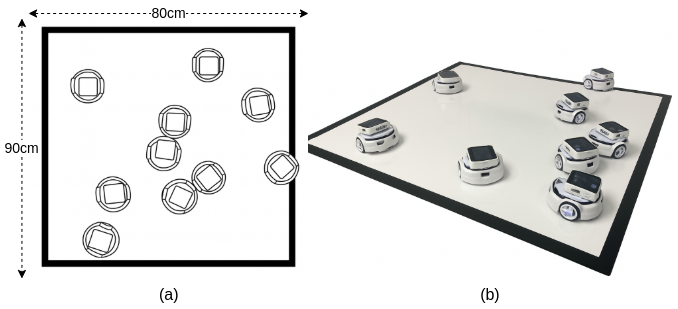
\includegraphics[width=0.49\textwidth]{arena.png}
    \caption{Robot Arena: (a) dimensions and (b) example of locomotion experiment with 8 robots.}
    \label{fig:arena}
\end{figure}

Across the study, we evaluated swarm performance under different communication and system configurations. Each experiment manipulates a specific independent variable while holding all other conditions constant. These include:\\

\begin{itemize}
  \item \textbf{Swarm density}: The number of agents deployed simultaneously, ranging from 2 to 13.
  \item \textbf{Locomotion mode}: Robots were either stationary (\emph{static}) or navigated using a \emph{Brownian motion} gait (Section \ref{sec:locomotion}).
  \item \textbf{Topology inference}: Message transmission priority was governed by either a \emph{STOCHASTIC} shuffle or a \emph{COMM\_AWARE} ranking strategy based on link quality metrics (Section \ref{sec:topology-inference}).
  \item \textbf{Message budget}: A token-bucket rate limiter controlled how frequently agents could transmit messages (Section \ref{sec:limited-rate}).
  \item \textbf{Transmission frequency}: Each message was optionally delayed by a random interval derived from the maximum observed peer latency to reduce potential network collisions (Section \ref{sec:transmission-frequency}).
\end{itemize}


\subsection{Rastrigin Function}

The Rastrigin function is defined as follows:

\begin{equation}\label{eq:rastrigin}
f_R(\mathbf{x}) = 10n + \sum_{i=1}^{n} \left(x_i^2 - 10\cos(2\pi x_i)\right)
\end{equation}

where $n$ is the number of dimensions, in this case the number of genes. Whereas, $x$ is the individual genome being evaluated. The function has a global minimum at \( f_R(\mathbf{x}) = 0 \) when $x = [0, 0, ..., 0]$ for all dimensions \cite{rucinski_impact_2010}. For the purpose of this study we used $n = 10$ and a solution bounded at $-5.12<=x_i<=5.12$.

\subsection{Robot Platform}\label{sec:robot_platform}
\begin{figure}[h]
    \centering
    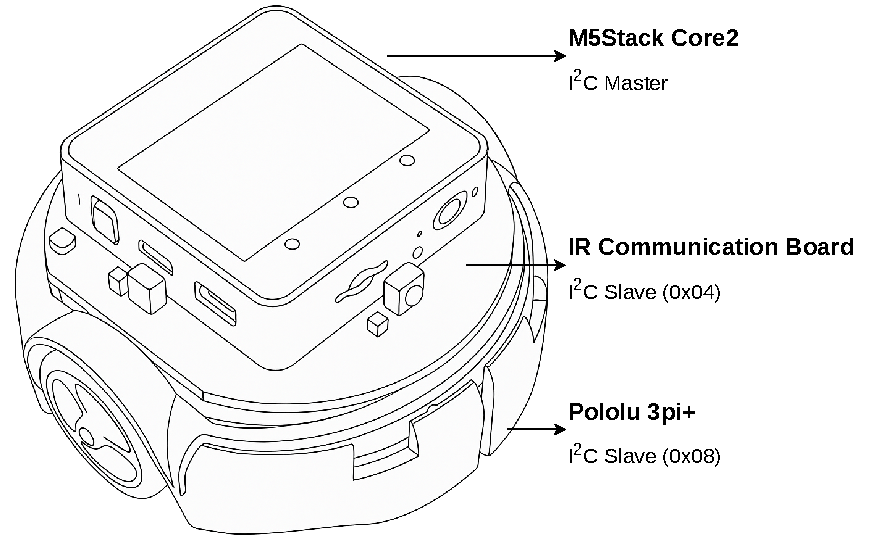
\includegraphics[width=0.45\textwidth]{B2.pdf}
    \caption{The Swarm-B2 platform: M5Stack Core2, IR Communication board, and Pololu 3Pi+}
    \label{fig:B2}
\end{figure}

Table~\ref{tab:B2-hardware} summarises the core hardware components of the Swarm-B2 platform used in this study [REF]. Coordination between devices is handled over a $I^2C$ 100kHz bus. Although the IR board can transmit and receive 32-byte frames, we did not conduct experiments with this feature. The board therefore behaves as a $I^2C$ bridge between the M5 and the Pololu 3Pi+. This guarantees that the communication results in this study stem only from a single data link.\\

\begin{table}[h]
  \centering
  \caption{Swarm-B2 hardware stack}
  \label{tab:B2-hardware}
  \begin{tabular}{p{0.18\linewidth} p{0.22\linewidth} p{0.42\linewidth}}
    \toprule
    Component & Interface(s) & Function \\
    \midrule
    M5Stack Core2 (240 MHz) & $I^2C$ master and SPI & Embodied evolution, ESP-NOW communication, data logging to SD and user interface \\
    IR board (16 MHz) & $I^2C$ slave (0x04) & Bus hub, optional IR feature \\
    Pololu 3Pi+ (16 MHz) & $I^2C$ slave (0x08) & Locomotion, bumper and line following sensors \\

    \bottomrule
  \end{tabular}
\end{table}

The ESP32 was used for running dual-core FreeRTOS parallel tasks, logging data on the local SD card and handling communication via the ESP-NOW data link (2.4 GHz). The 8MB PSRAM and larger flash memory on the master device allowed for concurrent task execution without peripheral starvation.\\

\subsubsection{Locomotion}\label{sec:locomotion}

The Pololu 3Pi+ is equipped with a line following sensor array and two bump sensors, which can be used to detect obstacles and detect the arena edges. A \emph{Brownian-motion} gait was selected to maintain unbiased mobility across the arena and ensure constant movement.\\

The gait code exposes the Pololu 3pi+ slave to the ESP32 master node, this interface lets the ESP32 act as a passenger with override, that can set wheel-speed scaling factors or raise \texttt{START}/\texttt{STOP} flags without touching the low-level control loop. In effect, the Pololu 3pi+ driver handles continuous motion, while the ESP32 decides when to go for each experimental condition.\\

\subsubsection{Local Data Storage}
We implemented local data logging mechanism (Section \ref{sec:data-logging}) on the ESP32 with a 16GB SD card peripheral. The shared SPI bus (with the LCD) was set at a frequency of 20MHz and configured to use the FAT32 file system for storage. This approach was chosen to emulate a realistic swarm system capable of operating remotely without relying on a stable Wi-Fi connection to a central server.\\

% Upon completing each run, the swarm members switch to a data upload mode and connect to the Wi-Fi, where the locally collected data is securely transmitted to an AWS S3 bucket using HTTPS. This might seem counter intuitive to our original objective, but it was planned to be this way as otherwise we would have to manually read each individual SD card to collect the data, which would be time consuming and error prone. Furthermore, we expect that in a real-world scenarios, the swarm would be deployed in a remote location where manual data collection would be impossible.\\

% Data logs are saved in the root directory of the SD card in a \.json format. Our system is designed to automatically generate new files upon reaching a specified size limit of 1MB, this enables efficient memory management and preventing heap memory overflow during log file writes.

\subsubsection{User Interface}

\begin{figure}[h]
    \centering
    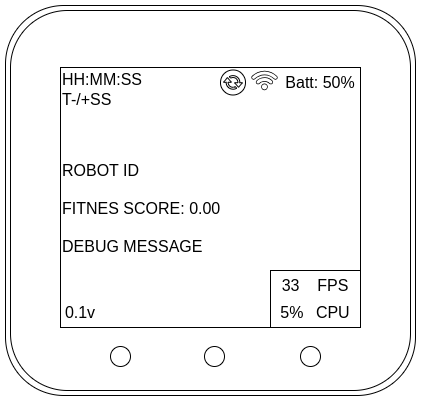
\includegraphics[width=0.35\textwidth]{UI.png}
    \caption{M5 user interface showing the current fitness score and device information.}
    \label{fig:UI}
\end{figure}

Figure \ref{fig:UI} shows the on-board user interface (UI) each Swarm-B2 agent displays during trials. A real-time clock (RTC) seeds a unique \emph{experiment\_id}, just below a $T\pm SS$ counter tells the operator how long until the next minute aligned run. Note that between peers there is an RTC's $\pm1$ drift, this is discussed in Section X. Status lines on the display list the robot's ID (last four hex digits of the MAC address), the live fitness score, and a single debug message. The bottom-left tag logs which software build is running on the device. Two icons round out diagnostics, the Wi-Fi symbol flashes during S3 log upload, and the circular arrow signals an over-the-air update.

\section{Implementation}

This section outlines the software design and implementation of the swarm firmware. The Espressif IoT Development Framework (ESP-IDF) was used as it provides low-level hardware access, offering greater flexibility for ESP-NOW communication (Section \ref{sec:comm-layer}). Unlike the Arduino framework, ESP-IDF provides direct access to FreeRTOS, enabling fine-grained control over concurrent task creation and dual-core processing, such as isolating communication tasks to a specific core. It also supports advanced features like over-the-air (OTA) updates (Section \ref{sec:ota}), unit testing, and custom debugging tools \cite{esp-boards_esp-idf_nodate}.

\subsection{Software Development Environment}\label{sec:SDK}

We employed a Continuous Integration and Continuous Deployment (CI/CD) pipeline via GitHub to automate OTA deployment, ensuring synchronized updates and easier debugging across the swarm (Fig. \ref{fig:cicd-architecture}).\\

The CI/CD integration proved especially valuable during experiments, where consistent updates across multiple agents were necessary. It also facilitated easier rollbacks in the event of unexpected bugs. The automated build pipeline in GitHub ensured that only validated firmware versions were propagated to the swarm, catching any environment discrepancies early in the process.\\

\begin{figure}[h]
    \centering
    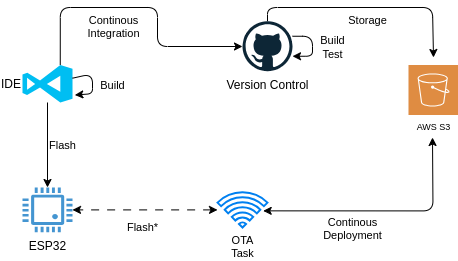
\includegraphics[width=0.45\textwidth]{architecture.png}
    \caption{CI/CD Architecture: Local development, GitHub repository, AWS S3 storage, and OTA updates.}
    \label{fig:cicd-architecture}
\end{figure}

Our software development framework for the swarm is as follows:

\begin{enumerate}
    \item \textbf{Local environment development}: Application development takes place locally using VSCode, our local environment uses version 5.1.4 of ESP-IDF and Python 3.11 to build and flash the code in-situ.\\
    \item \textbf{Version control}: We push updates of the codebase to a public repository on GitHub: \url{https://github.com/yallico/robotics_dissertation}, this allows for version control and triggers a custom build and test process. The ESP32 project is then compiled remotely and generates the binary file used for OTA.\\
    \item \textbf{Cloud storage}: The OTA binary file is uploaded to an AWS S3 public bucket making it accesible to the swarm via HTTPS.\\
\end{enumerate}

\subsubsection{OTA Process}\label{sec:ota}

Upon initialization, each agent checks its local firmware version against the latest version stored in S3. If a mismatch is detected, the ESP32 downloads and installs the updated .bin file. While relying on a central server and exposing the swarm to the internet for updates may seem counterintuitive, a similar update mechanism could be implemented in a decentralized manner using consensus protocols. However, this would have introduced additional complexity beyond the scope of this study.\\

\begin{table}[h]
  \centering
  \caption{System Partition Table}
  \begin{tabular}{l l l p{4.3cm}}
  \toprule
  \textbf{Name} & \textbf{Type} & \textbf{Size} & \textbf{Description} \\
  \midrule
  \texttt{nvs} & data & 16KB & Non-volatile storage \\
  \texttt{otadata} & data & 8KB & OTA metadata \\
  \texttt{phy\_init} & data & 4KB & PHY layer calibration data \\
  \texttt{factory} & app & 4MB & Default application \\
  \texttt{ota\_0} & app & 4MB & OTA slot 0 \\
  \texttt{ota\_1} & app & 4MB & OTA slot 1 \\
  \bottomrule
  \end{tabular}
  \label{tab:partition_table}
\end{table}


Table \ref{tab:partition_table} shows how each device partitions was configured with a dual-partition OTA scheme with two application slots: \texttt{ota\_0} and \texttt{ota\_1}. During an update, the new firmware is written to the inactive partition. Once the write and integrity checks pass, the bootloader switches to boot from the updated partition on the next reboot. This allows safe rollback in case of update failure. The update binaries ranged from 1 to 1.2 MB, note that update propagation and version control were managed manually through a quick check of the robot's LDC display before the experimental run.

\subsection{Embodied Evolution}

The swarm uses a distributed genetic algorithm (GA) to find the global minimum for Eq. \ref{eq:rastrigin}.A visual representation of this is shown in Fig. \ref{fig:ga}. As the local population in each agent evolves, the swarm begins to communicate their local best fitness and corresponding genes to their peers.\\

\begin{figure*}[t]
    \centering
    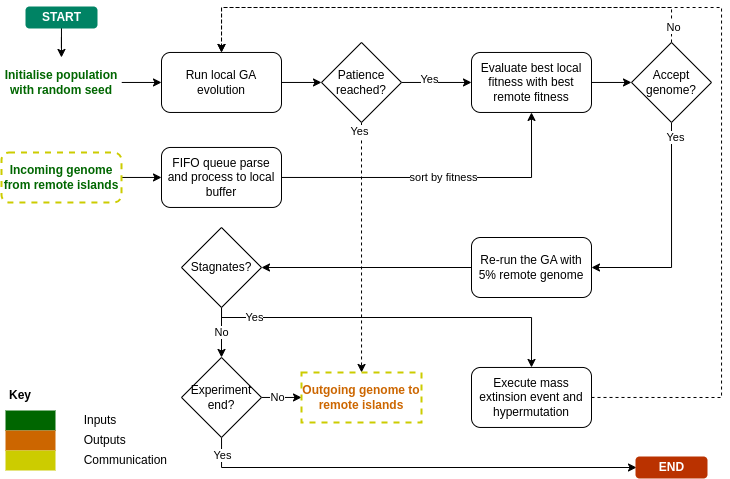
\includegraphics[width=0.65\textwidth]{ga.png}
    \caption{Island Model Flowchart}
    \label{fig:ga}
\end{figure*}

Our implementation employs an elitist migration strategy, this happens when the local GA reaches a patience threshold and the agent pushes its "best" (lowest fitness score) genome to other swarm members via ESP-NOW. The incoming remote genes from another peer are integrated into the local population by replacing the worst performing $5\%$ individuals, this value was chosen to preserve genomic high locally.\\ 

To avoid stagnation over a local-minimum, a mass extinction event together with a hyper-mutation mechanism tracks consecutive non-improving generations. Once a set of conditions is reached (Table X), the mutation probability is temporarily increased to escape local optima and lowest performing half of the population is re-initialised. This is done to promote exploration across the swarm and prevent premature convergence. 

\subsection{Real Time Operating System}

Each swarm member boots into a FreeRTOS runtime by calling \texttt{app\_main()}, which performs the initialisation of the following components: non-volatile storage, I2C peripherals, RTC, SD card, and ESP-NOW.

Figure \ref{fig:rtos} illustrates the sequence of these and their relation to the tasks that are spawned during run time. These tasks include:

\begin{itemize}
  \item \texttt{i2c\_task}: Handles communication with the $I^2C$ peripherals, including the AXP192 power supply, the IR board, the display and the Pololu 3pi+.
  \item \texttt{gui\_task}: Manages the UI on the M5Stack display, used for real-time feedback and debugging.
  \item \texttt{pololu\_heartbeat\_task}: Handles the $I^2C$ signal from the Pololu 3pi+, ensuring that the robot is operational and responsive.
  \item \texttt{ota\_task}: Manages OTA updates if a new version is available in S3 (Section \ref{sec:ota}).
  \item \texttt{espnow\_task}: Manages ESP-NOW communication between swarm members, handles message sending and receiving.
  \item \texttt{ga\_task}: Runs the local GA and coordinates with other tasks to log and transmit data.
  \item \texttt{write\_task}: Handles SD card operations, including data logging, managing file storage and uploading experimental results.
\end{itemize}

Following initialization, each robot enters the experiment phase explained in Algorithm \ref{alg:swarm-loop}. Using a random seed the initial local population for the GA is generated. The \texttt{ga\_task} then evolves the local population until 60 generations are reached without achieving a 0.01 decrease in population fitness. At which point the genome with the lowest fitness score is transmitted via ESP-NOW to remote peers. The \texttt{espnow\_task} then dequeues and parses all messages from the buffer, updating statistics and evaluating remote genomes with local genomes.\\

\begin{figure}[H]
    \centering
    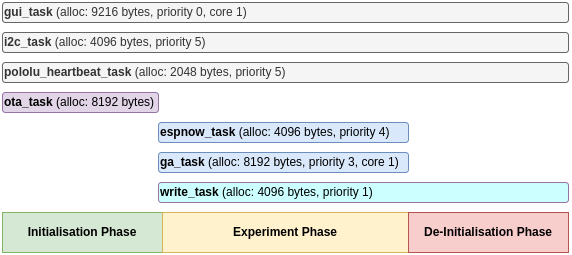
\includegraphics[width=0.48\textwidth]{rtos.png}
    \caption{Task schedule with memory allocation and priority.}
    \label{fig:rtos}
\end{figure}

Inter-task coordination is managed by event groups and queues. The event groups are used to signal task completion and synchronise downstream operations, whereas queues are used to pass data between tasks that are operating in parallel. This enables multitasking and real-time processing of the measurements.\\ 

Note that the local population undergoes evolution until the experiment phase is terminated. The experiment phase is terminated when one of the following criteria is met:

\begin{enumerate}
  \item \textbf{Global solution}: Any robot attains the exact global minimum of the Rastrigin function (fitness\,=\,0).
  \item \textbf{Time limit}: A maximum duration of 60 seconds elapses without global convergence.
\end{enumerate}

Upon reaching the de-initialisation phase, the \texttt{espnow\_task} drains pending message queues, final fitness and communication metrics are uploaded to an Amazon S3 bucket via HTTPS via the \texttt{write\_task}. Finally, the system peripherals are de-initialised to ensure a clean shutdown.

\begin{algorithm*}[h]
\caption{Experiment Phase Main Loop\label{alg:swarm-loop}}
\begin{algorithmic}[1]
  \State Generate random seed and initialise genetic algorithm population: \Call{init\_ga}{seed}
  \Loop
    \State \textbf{Check experimental phase:} \Call{ESPNOW\_COMPLETED\_BIT}{} \Comment{If set, proceed to de-initialisation phase}
    \State \textbf{Run GA:} \Call{evolve}{}
    \State Wait for GA completion flag \texttt{ga\_ended} \Comment{set in \texttt{ga\_complete\_callback}}
    \State \Call{espnow\_push\_best\_solution}{local\_genome}
    \State $ga\_has\_run\_before \gets \mathrm{true}$; $s\_last\_ga\_time \gets \mathrm{now\_ts}$
    \State \Call{drain\_buffered\_messages}{} \Comment{Dequeue all ESP-NOW frames}
    \ForAll{msg in \texttt{ga\_buffer\_queue}}
      \State \Call{parse\_out\_message}{msg} \Comment{Parse raw messages}
      \State \Call{ga\_integrate\_remote\_solution}{msg.genes}
    \EndFor
    \State \Call{check\_hyper\_mutation}{} \Comment{Apply if stagnation is detected}
    \State Reset \texttt{ga\_ended}
  \EndLoop
\end{algorithmic}
\end{algorithm*}

\subsection{Communication Layer}\label{sec:comm-layer}

We implemented ESP-NOW by pre-registering the MAC addresses for all peers in each agent, enabling direct unicast communication between swarm robots. Our design uses push only event-driven peer-to-peer messaging, where each device transmits data to peers without waiting for requests. Using this scheme avoids the complexity of pull-based communication protocols. Recall that once a local elite genome is found, the best solution is sent to all peers, if there are incoming messages these are queued for later processing, allowing task operations to continue uninterrupted. In this section we describe the specific communication independent variables that were manipulated during experiments.\\

% Using the IR board, described previously, the ESP32 was connected via the external $I^2C$ port. We had to use the Arduino library as a component of the ESP-IDF implementation for the this to work, this was due to compatibility issues between ESP-IDF and Arduino libraries. The board itself runs on a Arduino Nano to process the IR signals into messages and then sending this data accross via the SDA/SCL pins. One major implication for this, was the need to change the FreeRTOS clock speed from 100Hz to 1000Hz. Some key parameters also include the frequency if the I2C itself which was set at 100kHtz and the master/slave configuration, this is initialized from the M5 once powered on after the 5V bus is switched on.

\subsubsection{Topology Inference}\label{sec:topology-inference}

We investigate the impact of different communication schemes on the emergent swarm topology by introducing two distinct message transmission strategies: \textbf{STOCHASTIC} and \textbf{COMM\_AWARE}. Implemented in the communication layer, these were designed to influence the order and priority with which each agent sends data to its peers. The aim is to understand how these strategies affect the connectivity and robustness of the swarm network.\\

These are implemented as follows:

\begin{itemize}
    \item \textbf{STOCHASTIC}: Each agent calls a random seed to apply a Fisher-Yates shuffle over the list of peer MAC addresses to sort them before sending its message. This ensures that the order of communication is random for each transmission cycle, preventing biases.
    \item \textbf{COMM\_AWARE}: Each agent ranks its peers based on the most recent measurements of communication quality, specifically the last known latency and Received Signal Strength Indicator (RSSI). Peers with unknown metrics (during initialisation) are prioritized first to ensure all peer links are measured. Then, peers are scored by normalizing both latency and RSSI, and those only in the worst half (highest latency, lowest RSSI) are prioritized for message transmission.
\end{itemize}

The following pseudocode outlines the logic for each scheme:

%\paragraph{STOCHASTIC}
\begin{algorithm}[H]
\caption{Randomized Peer Selection}
\begin{algorithmic}[1]
\State \textbf{Input:} List of peer MAC addresses
\State Fisher-Yates shuffle using a random seed
\For{each peer in shuffled list}
    \If{peer is not self}
        \State Send message to peer
    \EndIf
\EndFor
\end{algorithmic}
\end{algorithm}

%\paragraph{COMM\_AWARE}
\begin{algorithm}[H]
\caption{Communication-Aware Peer Ranking}
\begin{algorithmic}[1]
\State \textbf{Input:} List of peer MAC addresses, last known RSSI and latency for each peer
\For{each peer}
    \If{RSSI or latency is null}
        \State Assign highest priority
    \Else
        \State Normalize RSSI and latency across all peers
        \State Compute score: $score = norm\_latency + norm\_rssi$
    \EndIf
\EndFor
\State Sort peers: null metrics first, then by descending score (worst first), only \textbf{50\% scope of network}
\For{each peer in sorted list}
    \If{peer is not self}
        \State Send message to peer
    \EndIf
\EndFor
\end{algorithmic}
\end{algorithm}

Note that these schemes are specifically designed for \textbf{unicast} communication, where messages are sent directly to individual peers and round-trip latency can be measured via acknowledgements (ACKS). Having said that, we can think of the \textbf{STOCHASTIC} algorithm as a pseuso-broadcast communication scheme as the message is sent to all peers with negligible delays between transmissions.\\ 

\subsubsection{Limited-Rate Communication}\label{sec:limited-rate}

Inspired by the “less-is-more” effects reported by \cite{aust_hidden_2022} using infrared links, we implemented a token-bucket limiter to the ESP-NOW layer and treat this quota as an independent variable. Each agent is given a small budget of 1 message in a sliding window of length 8 seconds.  When the bucket is empty the agent must keep silent until the window refreshes, regardless of how often its GA stagnates or improves.  This caps the total interaction rate per robot rather than solely spacing individual transmissions.

\begin{algorithm}[H]
\caption{Token-Bucket Throttled Send}
\label{alg:token_bucket}
\begin{algorithmic}[1]
\Require 
  $B$: message budget per window, \quad
  $W$: window length (ms), \quad
  $t_{\mathrm{last}}$: window start time, \quad
  $\mathit{tokens}$: remaining sends
\Procedure{MaybeSend}{$\mathit{payload}$}
  \State $now \gets$ \Call{CurrentTimeMs}{}
  \If{$now - t_{\mathrm{last}} \ge W$} \Comment{Window refresh}
    \State $\mathit{tokens} \gets B$
    \State $t_{\mathrm{last}} \gets now$
  \EndIf
  \If{$\mathit{tokens} = 0$}
    \State \Return \Comment{Bucket empty → no send}
  \EndIf
  \If{\Call{ImprovedFitness}{}}
    \State $\mathit{tokens} \gets \mathit{tokens} - 1$
    \State \Call{ESP\_NOW\_Send}{$\mathit{payload}$}
  \EndIf
\EndProcedure
\end{algorithmic}
\end{algorithm}

\subsubsection{Transmission Frequency}\label{sec:transmission-frequency}

To further explore the communication behaviour of the swarm under flooding conditions, we modulate the transmission frequency. In this communication mode, each message transmission is delayed by a random interval, otherwise no delay is explicitly applied. This random delay, drawn from a range determined by the maximum observed latency among peers, is described by Algorithm \ref{alg:transmission_freq}.\\

\begin{algorithm}[H]
\caption{Stochastic Transmission Frequency}
\label{alg:transmission_freq}
\begin{algorithmic}[1]
\State \textbf{Input:} List of peer MAC addresses, maximum latency observed ($max\_rand$)
\For{each peer in the target list}
    \If{peer is not self}
        \State Compute a random delay: $delay \gets rand(0, max\_rand)$
        \State Wait for $delay$ milliseconds
        \State Send message to peer
    \EndIf
\EndFor
\end{algorithmic}
\end{algorithm}

In the firmware, this is implemented by checking if \texttt{DEFAULT\_MIGRATION\_FREQUENCY} is set to \texttt{FREQUENCY\_RANDOM} and, if so, randomly delaying each call to \texttt{esp\_now\_send} by a value within the range of $[0, max\_rand]$, where $max\_rand$ is derived from the maximum measured latency among peers. The intention of this approach is to control the flooding of messages in a stochastic manner that can help reduce unintended collisions in the swarm network.

\subsection{Data Logging}\label{sec:data-logging}

Reliable and precise data logging is a pre-requisite for evaluating the communication performance and evolution dynamics of the swarm. To achieve this, our firmware implements several mechanisms to capture and record key metrics such as latency, message exchanges, internal state changes, and experiment metadata. These measurements are logged using well-defined data structures and are incrementally written to an SD card.\\

\subsubsection{Messaging Structure}

Table \ref{tab:out_message} summarizes the \texttt{out\_message\_t} structure used for transmitting messages between swarm peers via ESP-NOW. Note that any floating point values in the message content are rounded to $3 d.p.$ to ensure compact representation. The total size of the struct is kept within the raw payload limits (250 bytes) imposed by ESP-NOW to guarantee reliable transmission.

\begin{table}[h]
  \centering
  \caption{Message Structure (\texttt{out\_message\_t}) for ESP-NOW Data Transfer}
  \label{tab:out_message}
  \begin{tabular}{l l p{4cm}}
    \toprule
    \textbf{Field} & \textbf{Type} & \textbf{Description} \\
    \midrule
    \texttt{log\_id} & uint32\_t & Unique internal identifier of the event.\\
    \texttt{robot\_id[5]} & char & MAC identifier for the sender robot plus a null terminator.\\
    \texttt{created\_datetime} & time\_t & Timestamp based on the internal RTC.\\
    \texttt{message[128]} & char & Content of the message including the fitness score and genome delimited by "$|$".\\
    \bottomrule
  \end{tabular}
\end{table}

\subsubsection{Data Processing}

The data logging pipeline is designed to ensure that all key experimental metrics are captured and preserved locally by each agent. Log entries are posted to two FreeRTOS queues: \texttt{LogQueue} for internal logging events and \texttt{LogBodyQueue} for detailed message logs. A \texttt{QueueSet} allows the dedicated \texttt{write\_task} to efficiently monitor and process both queues in real time.\\

The core logging framework relies on three primary data structures:
\begin{itemize}
    \item \texttt{experiment\_metadata\_t}: Stores overall experiment parameters, including experiment and robot IDs, random seed, GA parameters, migration settings, and application version.
    \item \texttt{event\_log\_t}: Used for logging system events such as latency measurements, RSSI, CPU usage, and state changes.
    \item \texttt{event\_log\_message\_t}: Holds the parsed version of the \texttt{out\_message\_t} structure and links it to the internal event ID.
\end{itemize}

When an entry is retrieved from either queue, it is serialized into a JSON-formatted string (via \texttt{serialize\_log\_to\_json()}) to ensure structured and consistent downstream analysis. The serialized data is then written incrementally to SD card files, with each file capped at 1MB to prevent memory overflow and ensure robust storage. Figure~\ref{fig:data-store} illustrates the internal data logging pipeline, from event generation to SD card storage.

\begin{figure}[h]
    \centering
    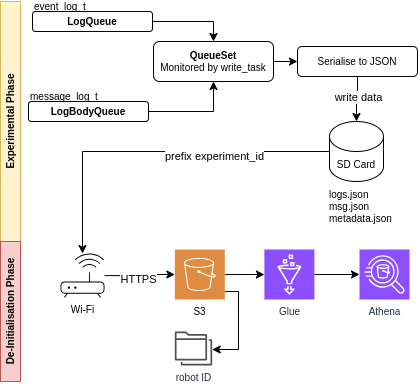
\includegraphics[width=0.45\textwidth]{data_store.png}
    \caption{Internal data logging pipeline}
    \label{fig:data-store}
\end{figure}

\subsection{Post-experimental Processing}

After the experimental phase concludes (Fig. \ref{fig:rtos}), the system enters a data upload mode. In this mode, the files stored on each agent's SD cards are uploaded to an AWS S3 bucket via HTTPS. This was done by design as we did not want to stream the data from the peers whilst they were running the experiment, as this could have introduced additional collisions potentially impacting the measurements.\\

\begin{figure}[H]
    \centering
    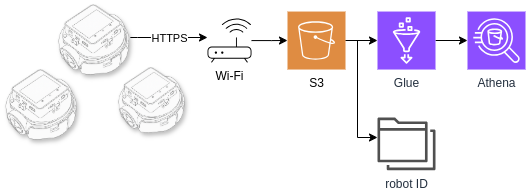
\includegraphics[width=0.45\textwidth]{athena.png}
    \caption{Data Upload Architecture}
    \label{fig:athena}
\end{figure}

As depicted by Figure \ref{fig:athena}, the S3 bucket is structured to store each agent's data in a separate folder, named by the robot's ID. Each file is named with a timestamp and the experiment ID, ensuring that all data is uniquely identifiable and traceable. The data is then processed using AWS Glue to prepare it for analysis in Amazon Athena. This process allowed us to automate the storage and evaluation of data logs from over $500$ experiment runs.\\

\section{Preliminary Sensitivity Analysis}

\begin{figure*}[h]
    \centering
    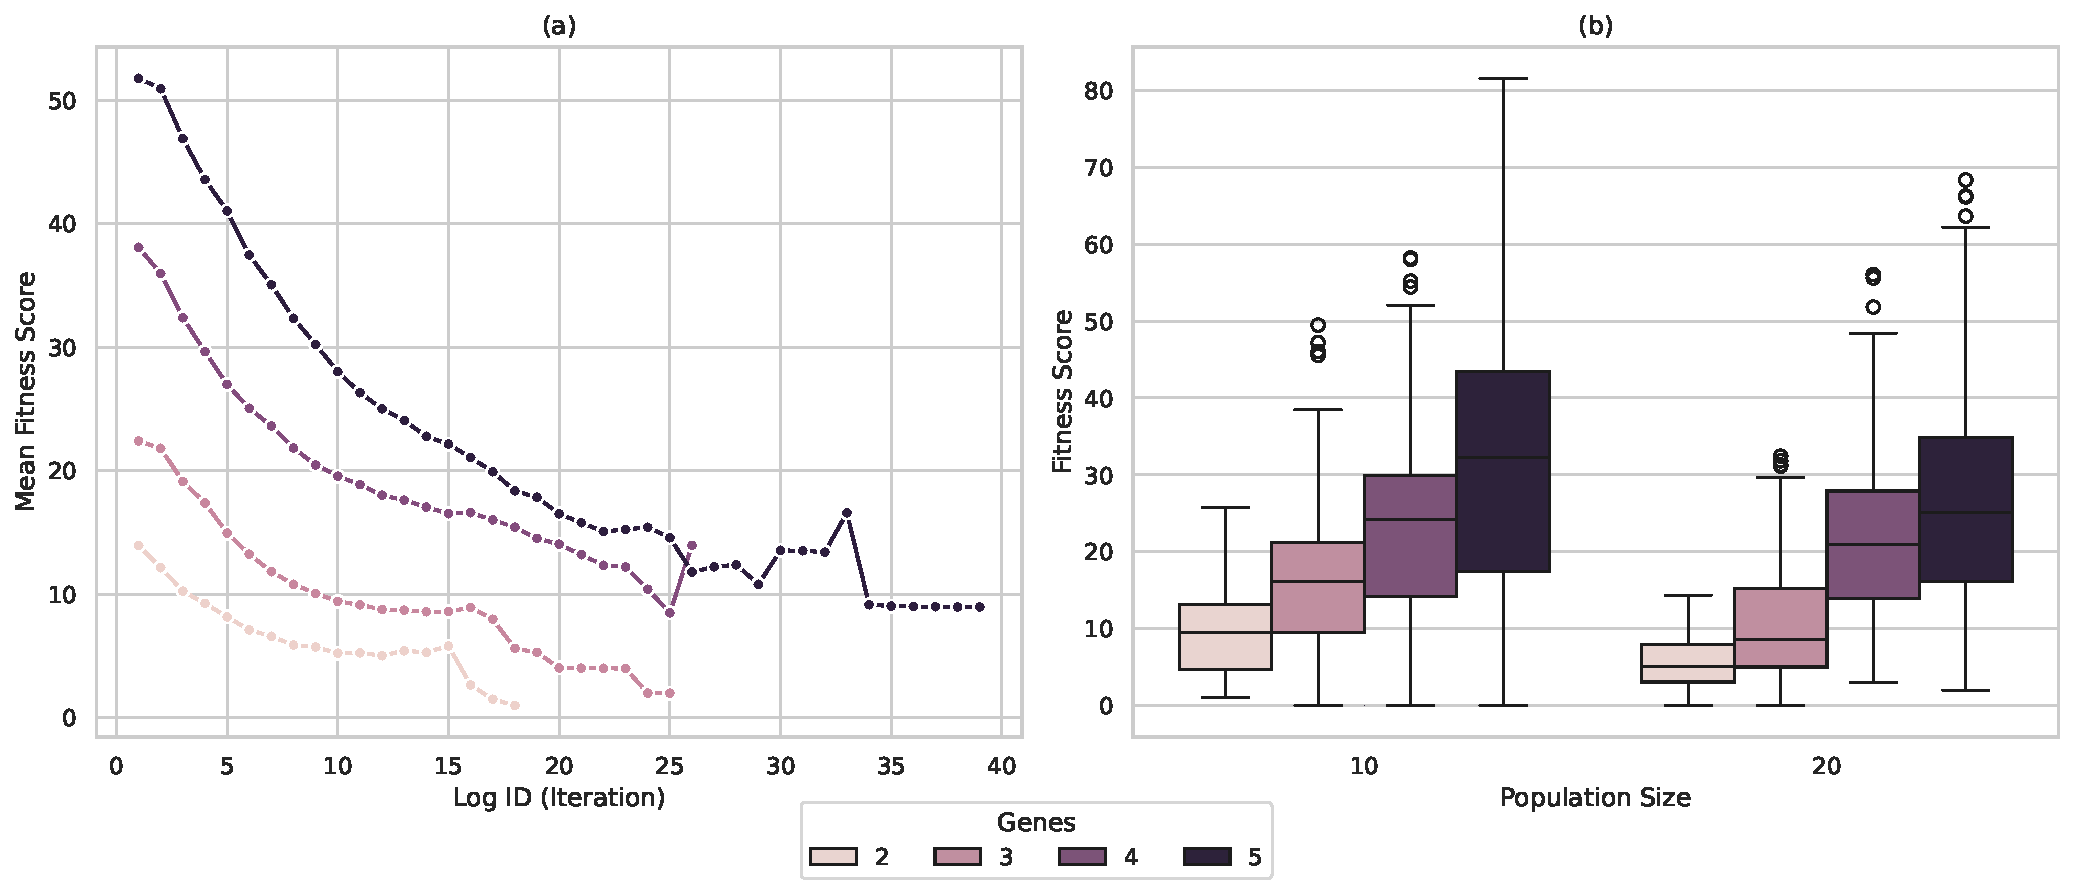
\includegraphics[width=1\textwidth]{ga_prelim_analysis.pdf}
    \caption{a: Number of iterations for algorithm to converge to either a global or local minimum. b: Fitness distribution by population size and genes.}
    \label{fig:ga_prelim_analysis}
\end{figure*}

Using a single robot, a preliminary analysis was conducted to identify suitable parameters for solving the Rastrigin function under varying population sizes (10, 20) and gene dimensions (2, 3, 4, 5). Over 100 experimental runs were performed, each terminating if fitness failed to improve beyond a 0.001 threshold over 20 consecutive epochs. Across all runs, the time taken to converge ranged between 0 to 3 seconds, reflecting the early stopping triggered by the patience setting. As shown in Figure~\ref{fig:ga_prelim_analysis}, larger populations yielded lower final fitness.\\

The data gathered from these early experiments suggested that using five genes was not sufficiently challenging for a single agent as convergence was achieved too quickly. Due to this we decide to expand the Rastrigin search dimentionality to 10 genes and extend the local population and threshold epochs to 60. Hypermutation parameters are also set at this stage and detertime that the most practical experiment run time of 60 seconds is appropiate for this configuration.

\section{Base Line Results}

\begin{figure*}[t]
  \centering
  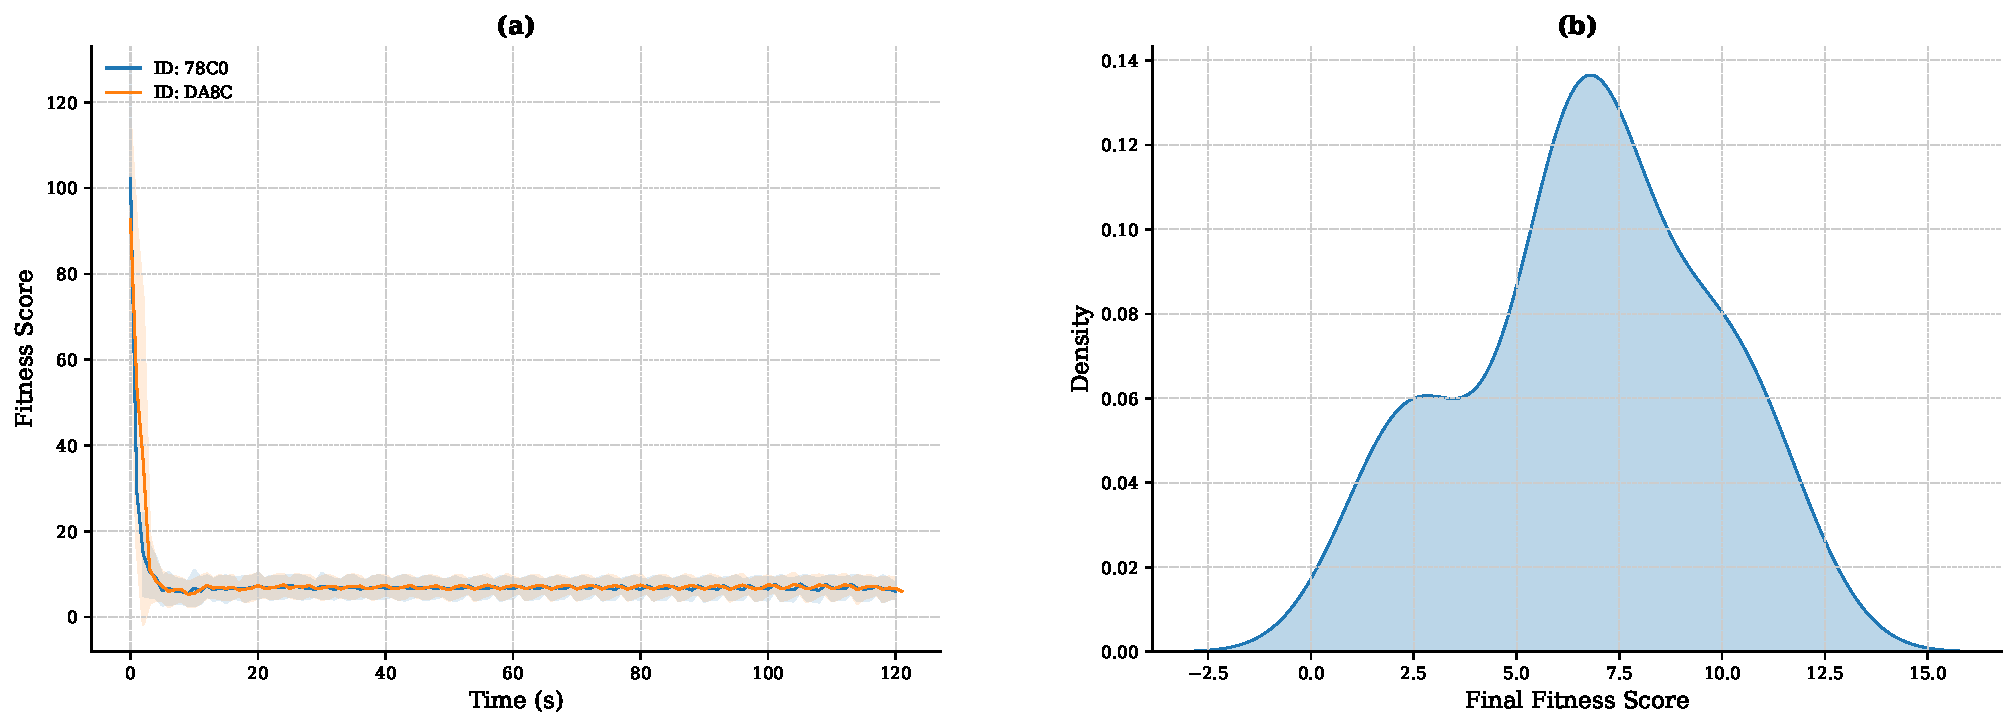
\includegraphics[width=1\textwidth]{base_fitness_stats.pdf}
  \caption{a: Mean population fitness score for each agent over time,  b: Final fitness score density distribution, c: Mean CPU utilisation over time.}
  \label{fig:base_fitness_stats}
\end{figure*}

Figure \ref{fig:base_fitness_stats} shows the fitness scores and system metrics for a deployment of two agents. A total of 34 experimens were conducted, out of which 6 experiments had to be excluded from the analysis as the data did not reach the S3 for at least one of the devices, mainly due to a bug in the code that was caused by the messages arriving late and the system not being able to handle these in the de-initiasation sequence. This bug was addressed since version 0.4 of the project, which allows the \texttt{espnow\_task} to drain the queue for any late messages coming in.\\

\begin{table}[h]
  \centering
  \caption{Baseline Configuration Parameters}
  \label{tab:base_config}
  \begin{tabular}{l@{~=~}l}
    app\_ver & 0.3\\
    data\_link & ESPNOW\\
    routing & unicast\\
    population\_size & 30\\
    max\_genes & 5\\
    patience & 30\\
    migration\_type & asynchronous\\
    migration\_scheme & elitist\\
    migration\_rate & 1\\
    migration\_frequency & patience based\\
    hyper\_mutation & true\\
    mass\_extinction & true\\
    robot\_speed & 0\\
    topology & fully connected\\
    experiment\_time & 120 s\\
  \end{tabular}
\end{table}

Using the baseline parameters shown in Table \ref{tab:base_config}, we can see that none of the experiments was able to reach the global minimun of 0.0 in terms of the fitness score. The mean final fitness score achieved was X.X indicating that a local minimum is reached, whereas the rate of the converge takes place within the first 10 seconds of the experiment and stagnates thereafter. This behaviour is aligns with a large CPU utilisation in both cores at the start of the experiment, from observations this can be attributed to the first local GA running in each agent which then stagnates after exchanging a few messages with the other peer. Taking this into consideration, for experiments from version 0.4 onwards the population size and number of genes are doubled to 60 and 10 respectively, to ensure diversity in the gene pool with the trade off of slower convergence.\\

\begin{figure*}[b]
  \centering
  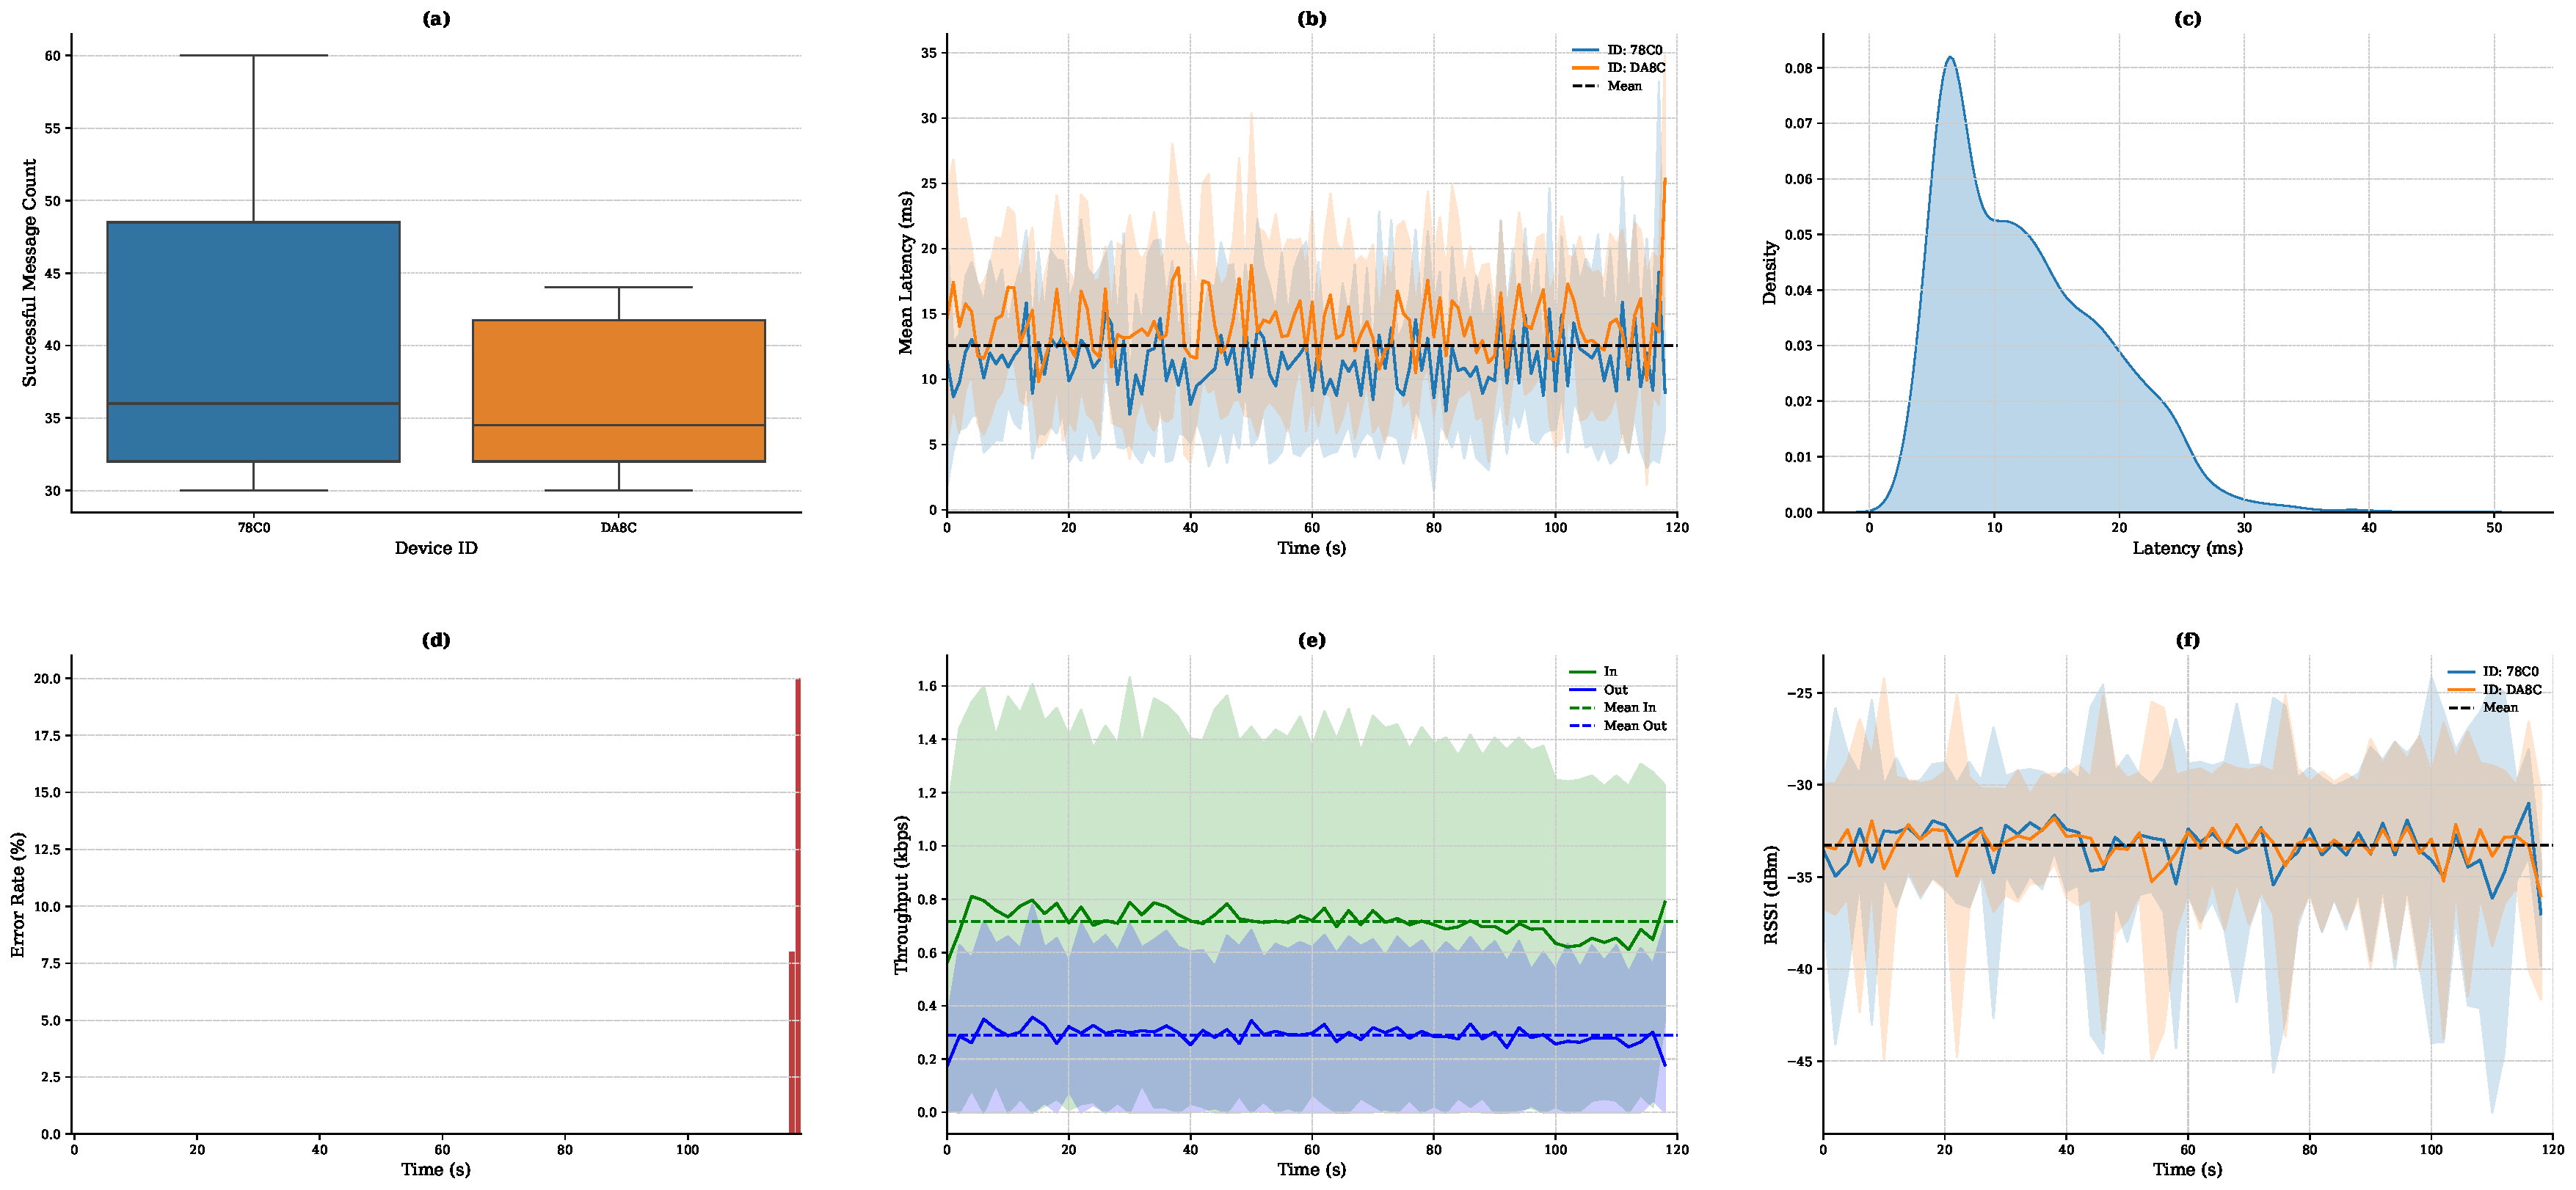
\includegraphics[width=1\textwidth]{base_comm_stats.pdf}
  \caption{a: Message sent distribution by each device,  b: Mean latency by device over time, c: Latency distribution accross all experiments, d: Mean error rate from failed messages over time, e: Mean throughput In/Out over time, f: Mean RSSI by device over time.}
  \label{fig:base_comm_stats}
\end{figure*}

Figure \ref{fig:base_comm_stats} shows the communication statistics for the same deployment of the two agents and the top level metrics are described in Table X. The mean latency was X.X ms, with a maximum latency of X.X ms. The latency statistics show that the ESPNOW protocol is able to handle the communication between the agents with low latency which is in line with other IoT applications REF. One artifact of the data worth noting is that high latencies were observed at the end of the experiments where the error rate was the highest, this is likely due to the longer delay in recieving an ACK from the other peer which has already de-initialised the ESPNOW task and is no longer able to respond to the messages. This would indicate that larger latencies are driven by failed messages pending an ACK. Note that in our base config we set the ESPNOW parameter \texttt{ESPNOW\_MAX\_RETRIES} to 0, which means that the messages are not retried if they fail to be sent. This is done to avoid having to handle pull type protocols which would involve having to handle requests and responses in a sequential manner.\\

\begin{table}[h]
  \centering
  \caption{Baseline Network Performance Metrics}
  \label{tab:baseline_network_metrics}
  \begin{tabular}{ll}
  \toprule
  \textbf{Metric} & \textbf{Value} \\
  \midrule
  Network Jitter (ms)      & 8.80  \\
  Max Bandwidth (kbps)     & 1.41  \\
  Network Error Rate (\%)  & 0.01  \\
  QoS (0--1)               & 0.7   \\
  \bottomrule
  \end{tabular}
\end{table}

The mean In/Out throughput achieved was X.X kbps and X.X respectively. It is worth noting that the higher In throughput suggests that there is an imbalance in the number of messages being exchanged, this can be confirmed by plot (a) in Figure \ref{fig:base_comm_stats} that shows one agent sending more messages than the other. This is likely due to the fact that the agents are not perfectly synchronised by the RTC, this means they finalise their first local GA at different times (also impacted by the random seed). This means that one agent is able to send its best solution before the other agent has a chance to send its own, this is an artifact of the current implementation and might have to be addressed in future work. Note that the expectation is that the network throughput will increase as the swarm increases in size, where the theoretical max throughput for ESPNOW is 214 kbps by device.\\ 

The mean RSSI accross all devices was X.X dBm, which in in a range that indicates that the communication link is stable and reliable REF. It is worth noting that the RSSI is measured between peers and therefore it can be used as an indicative measure of the distance between agents though we also expect that the RSSI will be affected by the environment and obstacles in between the agents. This influence will be explored in Section X where the topology of the swarm is varied to see how this affects the communication performance.\\

\section{Hypothesis}

%topology
The initial expectation is that both \textbf{STOCHASTIC} and \textbf{COMM\_AWARE} will result in a fully connected network over time, as each agent attempts to send messages to all other agents. However, the \textbf{COMM\_AWARE} scheme is designed to preferentially strengthen links with agents that are either furthest away (as inferred by higher latency and lower RSSI) or have not yet established a reliable connection (null metrics).\\ 

%moving bucket
By enlarging $W$ we progressively restrict social signalling, the following hypothesise are put forward:

%transmission
should in theory alleviate message collisions that can occur during the default pseudo-broadcasting mode of the swarm. By applying this stochastic delay on a per-peer basis, the system emulates a flooding mechanism with randomised inter-transmission intervals.

\begin{enumerate}
  \item \textbf{Convergence speed will decrease}: fewer migrations mean each island explores locally for longer before external influence arrives.
  \item \textbf{Task performance will improve}: reduced network contention and wider behavioural diversity should help the swarm escape local minima, yielding lower global Rastrigin scores by the termination time.
\end{enumerate}

Thus, the experiments tests whether the "less is more" phenomenon extends from low-bandwidth IR to high-bandwidth ESPNOW links.

\subsection{Experiment Schedule}\label{sec:experiments-schedule}

A minimum of 16 re-runs per condition was conducted to ensure statistical significance of the results.

\begin{table*}[H]
\centering
\label{tab:exp_config}
\caption{Experimental configurations}
\begin{tabular}{c|c|c|c|c}
\toprule
\textbf{Number of Robots} & \textbf{Topology Inference} & \textbf{Locomotion} & \textbf{Message Limit} & \textbf{Transmission Frequency} \\
\midrule
\multirow{10}{*}{3}
  & \multirow{5}{*}{Stochastic}
    & \multirow{2}{*}{Static}
                 & Unlimited& None \\
  &   &          & Unlimited& Random Delay \\
  &   &          & 1 msg/8s & None \\
  \cmidrule{4-5}
  &   & \multirow{2}{*}{Brownian}
                 & Unlimited& None \\
  &   &          & 1 msg/8s & None \\
  \cmidrule{2-5}
  & \multirow{5}{*}{Comm Aware}
    & \multirow{2}{*}{Static}
                 & Unlimited& None \\
  &   &          & 1 msg/8s & None \\
  \cmidrule{4-5}
  &   & \multirow{2}{*}{Brownian}
                 & Unlimited& None \\
  &   &          & 1 msg/8s & None \\
\midrule
\multirow{10}{*}{8}
  & \multirow{5}{*}{Stochastic}
    & \multirow{2}{*}{Static}
                 & Unlimited& None \\
  &   &          & Unlimited& Random Delay \\
  &   &          & 1 msg/8s & None \\
  \cmidrule{4-5}
  &   & \multirow{2}{*}{Brownian}
                 & Unlimited& None \\
  &   &          & 1 msg/8s & None \\
  \cmidrule{2-5}
  & \multirow{5}{*}{Comm Aware}
    & \multirow{2}{*}{Static}
                 & Unlimited& None \\
  &   &          & 1 msg/8s & None \\
  \cmidrule{4-5}
  &   & \multirow{2}{*}{Brownian}
                 & Unlimited& None \\
  &   &          & 1 msg/8s & None \\
\midrule
\multirow{10}{*}{13}
  & \multirow{5}{*}{Stochastic}
    & \multirow{2}{*}{Static}
                 & Unlimited& None \\
  &   &          & Unlimited& Random Delay \\
  &   &          & 1 msg/8s & None \\
  \cmidrule{4-5}
  &   & \multirow{2}{*}{Brownian}
                 & Unlimited& None \\
  &   &          & 1 msg/8s & None \\
  \cmidrule{2-5}
  & \multirow{5}{*}{Comm Aware}
    & \multirow{2}{*}{Static}
                 & Unlimited& None \\
  &   &          & 1 msg/8s & None \\
  \cmidrule{4-5}
  &   & \multirow{2}{*}{Brownian}
                 & Unlimited& None \\
  &   &          & 1 msg/8s & None \\
\bottomrule
\end{tabular}
\end{table*}

\section{Results}

\section{Discussion}
\textbf{COMM\_AWARE} scheme should result in a network where communication is dynamically biased towards improving weak or unmeasured links, using latency and RSSI as psuedo-metrics for distance allows the swarm to adapt to the percieved communication quality without having to know the exact positition of each member relative to itself. This is particularly useful in scenarios where the deployment is remote or there is no infrastructure available to track position. This communication schemes are only meaningful in swarms with more than two robots, as the benefits of dynamic peer selection and ranking emerge only in larger networks. \\

In the case of \textbf{BROADCAST} communication, it is not practical to measure per-peer latency, although RSSI can still be estimated by the receiver for each incoming message.
%need to decide if we will test broadcast....


% Add more chapters as needed

\newpage
\printbibliography

\end{document}